% Perl's replaceNode (Core/Document.pm:2011-2025) changes no box: its first replaceChild moves the
% replaced node into a document fragment, so removeNode finds no parent element whose box to
% update, and its closing appendNodeBox map runs over the @nodes its while(shift) loop emptied.
% The \@framebox afterConstruct unwraps its inner box through it (latex_constructs.pool.ltxml:4729;
% Rust sect12.rs), inside an auto-opened svg:foreignObject (a tikz node) or ltx:picture (\put).
% W12's first replace_node took the frame's box out of the auto-opened parent and put the inner
% box's in: the frame's padding and rule vanished from the sizes.
% witness: W12 review (orchestrator probes t3/t4/t5, 2026-09-25)
% oracle:  same-host Perl latexmlc (px, width x height / flip): 23.52x20.67/15.97 (fo, $x^2$);
%          33.7x42.62/24.77 (fo, tabular); 19.02 high /14.31 (fo, \parbox); 61.68x35.47 (picture)
% engines: rust (W12 2d49133036) = 14.12x11.26/11.26; 24.29x33.21/20.06; 9.61/9.61; 52.27x28.75
% expect:  0 errors; sizes as in Perl (the fo widths 23.53 and 78.73 are pre-W12 Rust: rounding,
%          and the \parbox fo width, 88.15 in Perl)
% status:  GREEN (56jo, W12; guard node_box_append::replacing_a_node_keeps_the_boxes)
\documentclass{article}
\usepackage{tikz}
\begin{document}
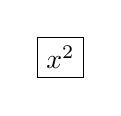
\begin{tikzpicture}\node {\fbox{$x^2$}};\end{tikzpicture}

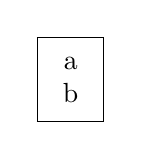
\begin{tikzpicture}\node {\fbox{\begin{tabular}{c}a\\b\end{tabular}}};\end{tikzpicture}

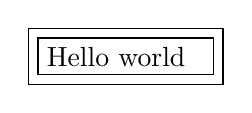
\begin{tikzpicture}\node[draw] {\fbox{\parbox{2cm}{Hello world}}};\end{tikzpicture}

x \put(0,0){A} \fbox{\vbox{\hbox{B}\hbox{CCC}}} y
\end{document}
